\chapter{Experimentos e Resultados}
\label{experimentos}

Ao fim do processo evolutivo do ICA, que parou por alguma das condições de parada implementadas, obtém-se os atributos do melhor país para se gerar um mapa de previsão futura, que mantém os aspectos de crescimento médio. E então define-se uma região de provável expansão para o mapa matriz, neste caso, partição do mapa matriz, com a aplicação de uma operação semelhante à utilizada na função de avaliação, removendo as partes dos cálculos de erro, mas mantendo o processo de previsão, que faz as convoluções e ponderações para gerar o mapa de previsão final.

A previsão gerada pelo método proposto pode ser comparada com um modelo estatístico que gera uma previsão sobre a curva de tendência linear também para cada região, de modo que cada região apresente uma taxa de crescimento seguindo a curva de tendência, onde cada quadrícula da região cresce homogeneamente, sem que haja a aplicação de nenhuma heurística, e seja usado apenas o modelo estatístico. Desta forma é possível comparar a precisão do modelo de previsão proposto região por região.

\subsection{Modelagem do ambiente}
\label{Exp:Modelagem do ambiente}

Neste trabalho, os dados foram selecionados utilizando a cidade de Taubaté-SP como região base para a criação dos mapas de quadrículas. Os dados contidos no banco de dados são referentes aos períodos de 2008 a 2015. Tais dados são separados de modo que cada período represente 1 ano, assim existirão inicialmente 8 arquivos de entrada para a aplicação, que transformará estes arquivos em mapas de quadrículas, que por sua vez serão particionados em várias pequenas partições para o processamento pelo ICA. 

Para que o método seja validado, devem ser usadas apenas uma porção dos dados para se gerar os países, e então usa-se o restante dos dados reais para se comparar com os dados de previsão computados após a etapa de evolução. Então pode-se separar a validação em duas etapas, sendo a primeira a etapa de treino, a qual se usa o ICA para evoluir os países sobre uma porção dos dados, e a segunda sendo referente à comparação entre os dados reais que não participaram do processo de evolução e os dados de previsão, gerados a partir dos países evoluídos. 

Assim, são selecionados os 5 primeiros anos, de 2008 a 2012, como \emph{nLearn} períodos de treino para o ICA, restando os 3 últimos anos, sendo 2013, 2014 e 2015, como \emph{nTest}, para testar e validar a metodologia de previsão. Neste caso, assim que se termina a etapa de evolução dos indivíduos, obtém-se o melhor indivíduo para aquela partição, e então geram-se 3 previsões seguidas a partir deste país, as quais serão comparadas com os mapas dos períodos reais restantes. A semelhança entre os mapas reais e previstos, devem seguir o crescimento definido pela curva de tendência gerada a partir dos períodos de teste, de modo que a previsão tenha seu crescimento seguindo a média padrão de crescimento entre os anos para que tal previsão seja validada e mais próxima possível do real.

Os mapas gerados de diversos períodos da cidade de Taubaté estão limitados nas latitudes \(Norte = -22.963715\) e \(Sul = -23.099506\) e nas longitudes \(Leste = -45.493534\) e \(Oeste = -45.674465\). O tamanho para cada lado das quadrículas é de 100 \(m\), resultando em uma área de 100 \(m^2\), sendo que tais áreas englobem aproximadamente de 1 a 4 quarteirões residenciais em média. Assim, os mapas ficam com altura igual a 150 quadrículas e largura igual a 185 quadrículas, o qual nos leva a ter que a região representa um retângulo de 18.5 \(km\) de largura por 15 \(km\) de altura, tendo uma área total de 277.5 \(km^2\). 

Estes mapas ainda são particionados em 15 partes para largura e para altura, gerando 210 partições de 13 x 10 quadrículas, sendo que as últimas 15, referentes às últimas colunas de cada linha sempre tenham dimensões 17 x 10 quadrículas para que não haja perda de informação ou geração de ruído em regiões não que estejam fora da definição \((Norte, Sul)\) e \((Leste, Oeste)\). Como cada quadrícula possui lado igual a 100 \(m\), tem-se que cada partição irá abranger uma área de 1300\(m\) X 1000\(m\) = 1300000\(m^2\) = 1.3\(km^2\) para as 210 quadrículas e 1700\(m\) X 1000\(m\) = 1700000\(m^2\) = 1.7\(km^2\)  para as 15 quadrículas restantes.

O tamanho das quadrículas foi diminuído, segundo \citeauthor{willis2002spatial}, o ideal é usar o tamanho das quadrículas como sendo \(\frac{1}{4} milha\), o que é aproximadamente 400\(m\) (\(\frac{1}{4} milha = 402.3360m\)), a fim de se aumentar a resolução de cada partição para que esta possa captar características mais bem definidas sempre que efetuar a metodologia de previsão sobre a partição. Caso fosse utilizado o tamanho da quadrícula original, igual a 400\(m\), cada partição seria composta por aproximadamente \(3 \times 2\) quadrículas, diminuindo assim a resolução de cada partição. Esta diminuição tem como intuito fazer com que cada quadrícula represente aproximadamente de 1 a 2 quarteirões de tamanho médio.

\subsection{Testes sobre cada região}
\label{Exp:Testes sobre cada região}

Não se foi definida uma relação entre o tamanho de cada partição e o tamanho da máscara de convolução, porém espera-se que cada partição seja pelo menos 2 vezes maior que a matriz de convolução tanto em largura quanto em altura para que as máscaras possam gerar mapas que possuam características da região abordada nesta região de uma forma aproximada sem que os valores mais periféricos da máscara fiquem, em sua maior parte durante o processamento, para fora da região a ser analisada. 

Sendo assim máscaras de ordem 3, 5 e 7 podem ser usadas para gerar as previsões para este caso, onde tem-se que a menor partição é de \(13 \times 10\) quadrículas, já as máscaras  de ordem 9, estão no limite entre o que se considera previsão com erro aceitável, podendo apresentar resultados de previsão não aceitáveis, e as máscaras de ordem 11, 13, etc. apresentam um resultado mais agressivo (mesmo aumentando o número de ponderações), já que alguns de seus valores mais periféricos ficarão para fora da imagem por muitos ciclos do processo de convolução, e assim, o ICA é incapaz de evoluir seus valores para alguma característica da região, de modo que a previsão de algumas regiões resulte em uma previsão irreal, \emph{estourando} a previsão de crescimento da região, tal que estes valores que ficam durante muitos ciclos de fora da região sejam em sua maior parte aleatórios, aplicando as características inexistentes na região de uma forma muito intensa em pontos mais distantes, gerando muito ruído no processo de previsão. 

A Figura \ref{fig:ForecastingSpike} mostra uma região real, e a mesma região com a previsão 'estourada'. As cores das regiões em questão foram invertidas para facilitar a visualização das áreas urbanas, neste caso pontos mais claros representam pontos de alta densidade e regiões mais escuras representam pontos de baixa densidade, a cor preta representa uma região com nenhuma residência.

\begin{figure}[h]
	\centering	
    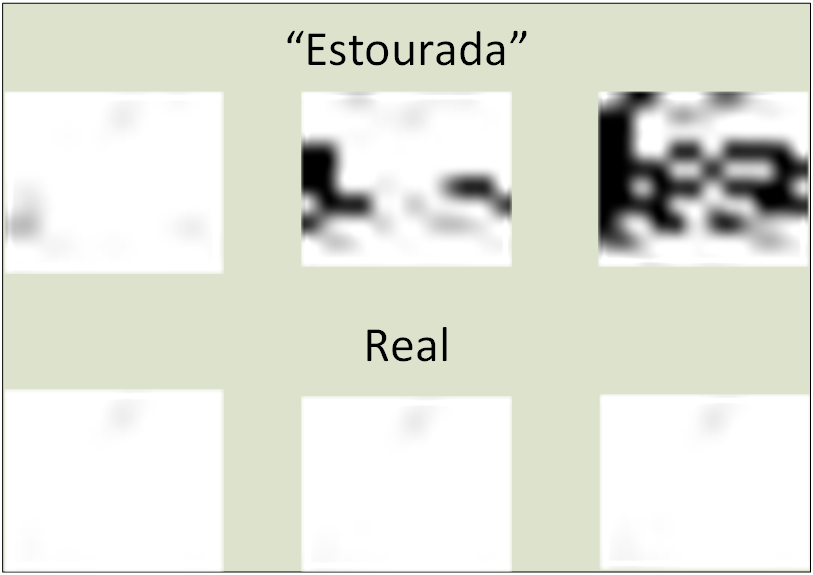
\includegraphics[scale=1]{Figuras/Image-PrevisaoEstourada.png}
	\caption{Imagem da previsão estourada}
	\label{fig:ForecastingSpike}
\end{figure}

Uma solução para este problema seria alterar o algoritmo de convolução para efetuar um processo de convolução aperiódica, que é uma forma diferente do padrão(convolução truncada, que centra a máscara com o primeiro pixel da imagem, e atribui zero aos valores inexistentes da imagem), que sempre agirá dentro da imagem porém atribui zero para resultados não calculáveis. A Figura \ref{fig:convApvsTr} abaixo ilustra no seu item \emph{(a)} a convolução aperiódica, e em \emph{(b)} a convolução padrão (Truncada).

\begin{figure}[h]
	\centering	
    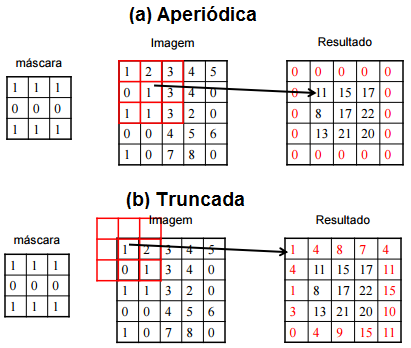
\includegraphics[scale=1]{Figuras/ConvolucaoAperiodica.png}
	\caption{Convolução aperiódica versus truncada}
	\label{fig:convApvsTr}
\end{figure}

A opção de utilizar esta forma de convolução não se aplicaria para a previsão, pois estaria-se perdendo informação e aumentando o erro da previsão de uma forma drástica, sendo que os valores das bordas de cada região seriam 0.


\subsection{Testes sobre todas regiões}
\label{Exp:Testes sobre todas regiões}


Para cada partição, será gerado um país através do processamento no ICA, que por sua vez será usado para fazer a previsão dos \emph{nTeste} períodos desta partição. Foram  executadas duas configurações de treino, sendo a primeira com apenas a condição de paradas por máxima quantidade de décadas, com os valores do ICA configurados como:

\begin{itemize}
\item Vetor de atributos do país:

  \begin{itemize}
  \item Os valores de fator estão limitados em [-50,50];
  \item Os valores das matrizes de convolução são estão limitados em [-100,100];
  \end{itemize}

\item valores das propriedades do ICA:

  \begin{itemize}
  \item Beta: 2;
  \item Taxa de revolução: 0.99;
  \item Taxa de decaimento de revolução: 0.999999;
  \item Taxa de impérios iniciais: 15\%.
  \item É Paralelo? sim;
  \item População inicial: 64;
  \item Máximo de décadas: 2048;
  \item Modo de movimento: Combinado(Refinado + Visão Imperial Distorcida);
  \end{itemize}

\end{itemize}

Para a segunda configuração, foi implementada uma condição de parada que leva em consideração o número máximo de décadas e o custo mínimo a ser atingido. Esta condição de parada segue o padrão de validação segundo o algoritmo \ref{alg:FpCP} apresentado abaixo:
	
 \begin{algorithm}[h]
\SetAlgoLined
\KwData
{
\\ \emph{curD} - década atual.
\\ \emph{maxD} - número máximo de décadas.
\\ \emph{curC} - custo do melhor país.
\\ \emph{minC} - valor do custo mínimo.
}
\KwResult{ 
\\ retorna se a condição de parada foi atingida ou não. 
}
	\Se{$curD$ >= $maxD$ * 10} 
    {
    	\KwRetorna Condição de parada atingida\;
    }
    \Se{$curD$ > $maxD$}
    {
    	\Se{$curC$ < $minC$}
     	{
        	\KwRetorna Condição de parada atingida\;
        }
    }
   \KwRetorna Condição de parada NÃO atingida\;

 \caption{Algoritmo condição de parada para o ICA}
\label{alg:FpCP}
\end{algorithm}

Observa-se no algoritmo da condição de parada que ela só será atingida quando atingir 10 vezes o número de máximo de décadas estipulado ou quando o custo for menor que \emph{minC} e, inclusivamente, o número de décadas for maior que o número máximo de décadas estipulado. Assim, garante-se que o algoritmo só irá parar segundo estas condições, tal que considera-se importante atingir o valor \emph{maxD} de décadas mesmo se o custo for menor que o valor definido em  \emph{minC}, e ainda tenta-se atingir \emph{minC} até 10 vezes o valor estipulado em \emph{maxD}. É importante mencionar que se um país chegar ao custo zero, o ICA para imediatamente, por este ser o melhor país (melhor solução a ser encontrada), e ainda, esta condição não é avaliada junto das condições de parada, mas sim antes de começar tal avaliação.

Esta segunda configuração não difere muito da primeira em questão dos parâmetros do ICA, basicamente insere-se esta nova condição de parada, que fica como:

\begin{itemize}
\item Vetor de atributos do país:

	\begin{itemize}
	\item mesmos valores;
	\end{itemize}

\item valores das propriedades do ICA:

	\begin{itemize}
	\item mesmos valores;
	\item Adicionar condição de parada 	padrão por número máximo de décadas: Não; 
	\item Usar condição de parada por década e Custo: Sim;
	\item Condição de parada adicional (por década e custo):

		\begin{itemize}
		\item Custo mínimo = 50;
		\item Máximo de décadas = 2048;
		\end{itemize}

	\end{itemize}

\end{itemize}

Geralmente, os países não convergem para custo 0, mas geram mapas com uma diferença mínima entre os períodos, de modo que este país quando utilizado para fazer uma previsão futura, seguirá o padrão de crescimento, elevando os valores de cada quadrícula de acordo com a função de testes descrita, que neste caso é a própria função que faz a previsão da expansão urbana, que usa o país como solução ótima aplicada sobre os dados, operando a ponderação das convoluções e gerando um mapa final de previsão.

Esta segunda configuração, apesar de parecer mais rápida, acaba sendo mais demorada por permitir que o número máximo de décadas se estenda para 10 vezes o tamanho configurado inicialmente. Porém, obtém-se uma previsão mais precisa em troca de tempo de processamento.

Em posse dos melhores países para cada partição, inicia-se o processo de geração dos \emph{nTest} mapas de previsão, também para cada partição. Assim que os mapas de previsão para cada partição são gerados, pode-se compará-los com com os mapas particionados reais, tomando a diferença absoluta entre a soma das diferenças das quadrículas (ou \emph{pixels}) dos mapas como sendo o erro de previsão daquela partição. 

Ao considerar cada partição como um bloco fechado, que cresce em densidade durante os períodos, tal bloco deve seguir uma linha de crescimento tendenciosa, que define em quantidades absolutas como tal bloco se desenvolverá durante períodos futuros. Mas é impossível saber, dentro deste bloco, onde e como tal crescimento será imposto. A linha de tendência sobre o crescimento do bloco fornece apenas um valor unitário de intensidade sobre como tal bloco se desenvolverá no futuro, de modo que só se pode afirmar, que todos os pontos (\emph{pixels} ou quadrículas) deste bloco irão crescer de um valor x para um valor x+y, seguindo especificamente a função de crescimento gerada pela curva de tendência linear. 

O modelo proposto, então apresenta uma solução para que se possa obter tal nível de precisão, de modo que os blocos, tenham um crescimento que siga tal linha de tendência, mesmo que a função de avaliação não os considere, e que além disso, apresentem uma solução que leve em consideração os pontos contidos no bloco, suas posições, intensidades e características regionais, dentro deste bloco, e portanto possibilitando a construção de um mapa de quadrículas disposto bidimensionalmente em forma de uma imagem, onde cada quadrícula pode ser representada por um pixel dessa imagem. Assim a análise de previsão desta metodologia utiliza-se de dois parâmetros para comparar a previsão, sendo o crescimento geral da região durante os períodos e o valor absoluto de acerto ponto a ponto.

Dentro deste cenário foram efetuados diversos testes, variando o tamanho da matriz de convolução, e a quantidade de ponderações. Foi definido que o número de ponderações igual a 3 é suficiente para prover suavidade e precisão no mapa de previsão gerado em relação aos métodos convencionais para geração do mapa de previsão. O uso de apenas um fator e uma matriz de convolução pode resultar algumas vezes, em um mapa de previsão semelhante ao modelo estatístico, que usa a curva de tendência (neste caso qualquer que seja, linear, exponencial, polinomial etc.) referente ao crescimento da região, mas não é tão preciso quando refere-se à constituição (forma e intensidade dos pontos) do mapa, relativo a quantidade de pontos, seja ela percentual ou absoluta, acertados pela previsão. O ponto negativo é que quanto mais ponderações houver, mais aumenta o uso de processamento, colocando mais precisamente, a quantidade de convoluções que aumenta de acordo com o número de ponderações, sendo que a operação de convolução é o processo mais pesado que ocorre durante a avaliação, que por sua vez aumenta o tempo de execução de todo o processo de avaliação.

O aumento da ordem da matriz de convolução aumenta drasticamente o tempo de processamento, porém traz resultados mais interessantes. Quando seleciona-se o tamanho mínimo de 3 para a ordem da matriz de convolução, os resultados apresentados já são satisfatórios e apresentam uma precisão no acerto sobre o crescimento geral da região e sobre a quantidade de acertos ponto a ponto melhor que a curva de tendência aplicada sobre a mesma região. Ao aumentar a ordem da matriz de convolução para 5, tem-se uma melhora no erro do crescimento da região em relação à matriz de ordem 3, porém aumenta-se sutilmente o erro da previsão ponto a ponto. Aumentando a ordem da matriz para 7, algumas regiões passam a apresentar um comportamento atípico, fazendo com que o resultado final de previsão exploda para valores de erros, tanto no crescimento regional geral quanto no ponto a ponto, muito maiores que os apresentados pelo modelo estatístico, tornando o mapa final de previsão muito ruidoso e impossível de ser usado para fazer qualquer tipo de análise. A Figura \ref{fig:allResults} mostra uma comparação entre os valores reais, os resultados gerados pela metodologia de previsão proposta, usando matrizes de convolução 3x3, 5x5, 7x7, com o modelo estatístico, para os anos de 2013, 2014 e 2015.

\begin{figure}[h]
	\centering	
    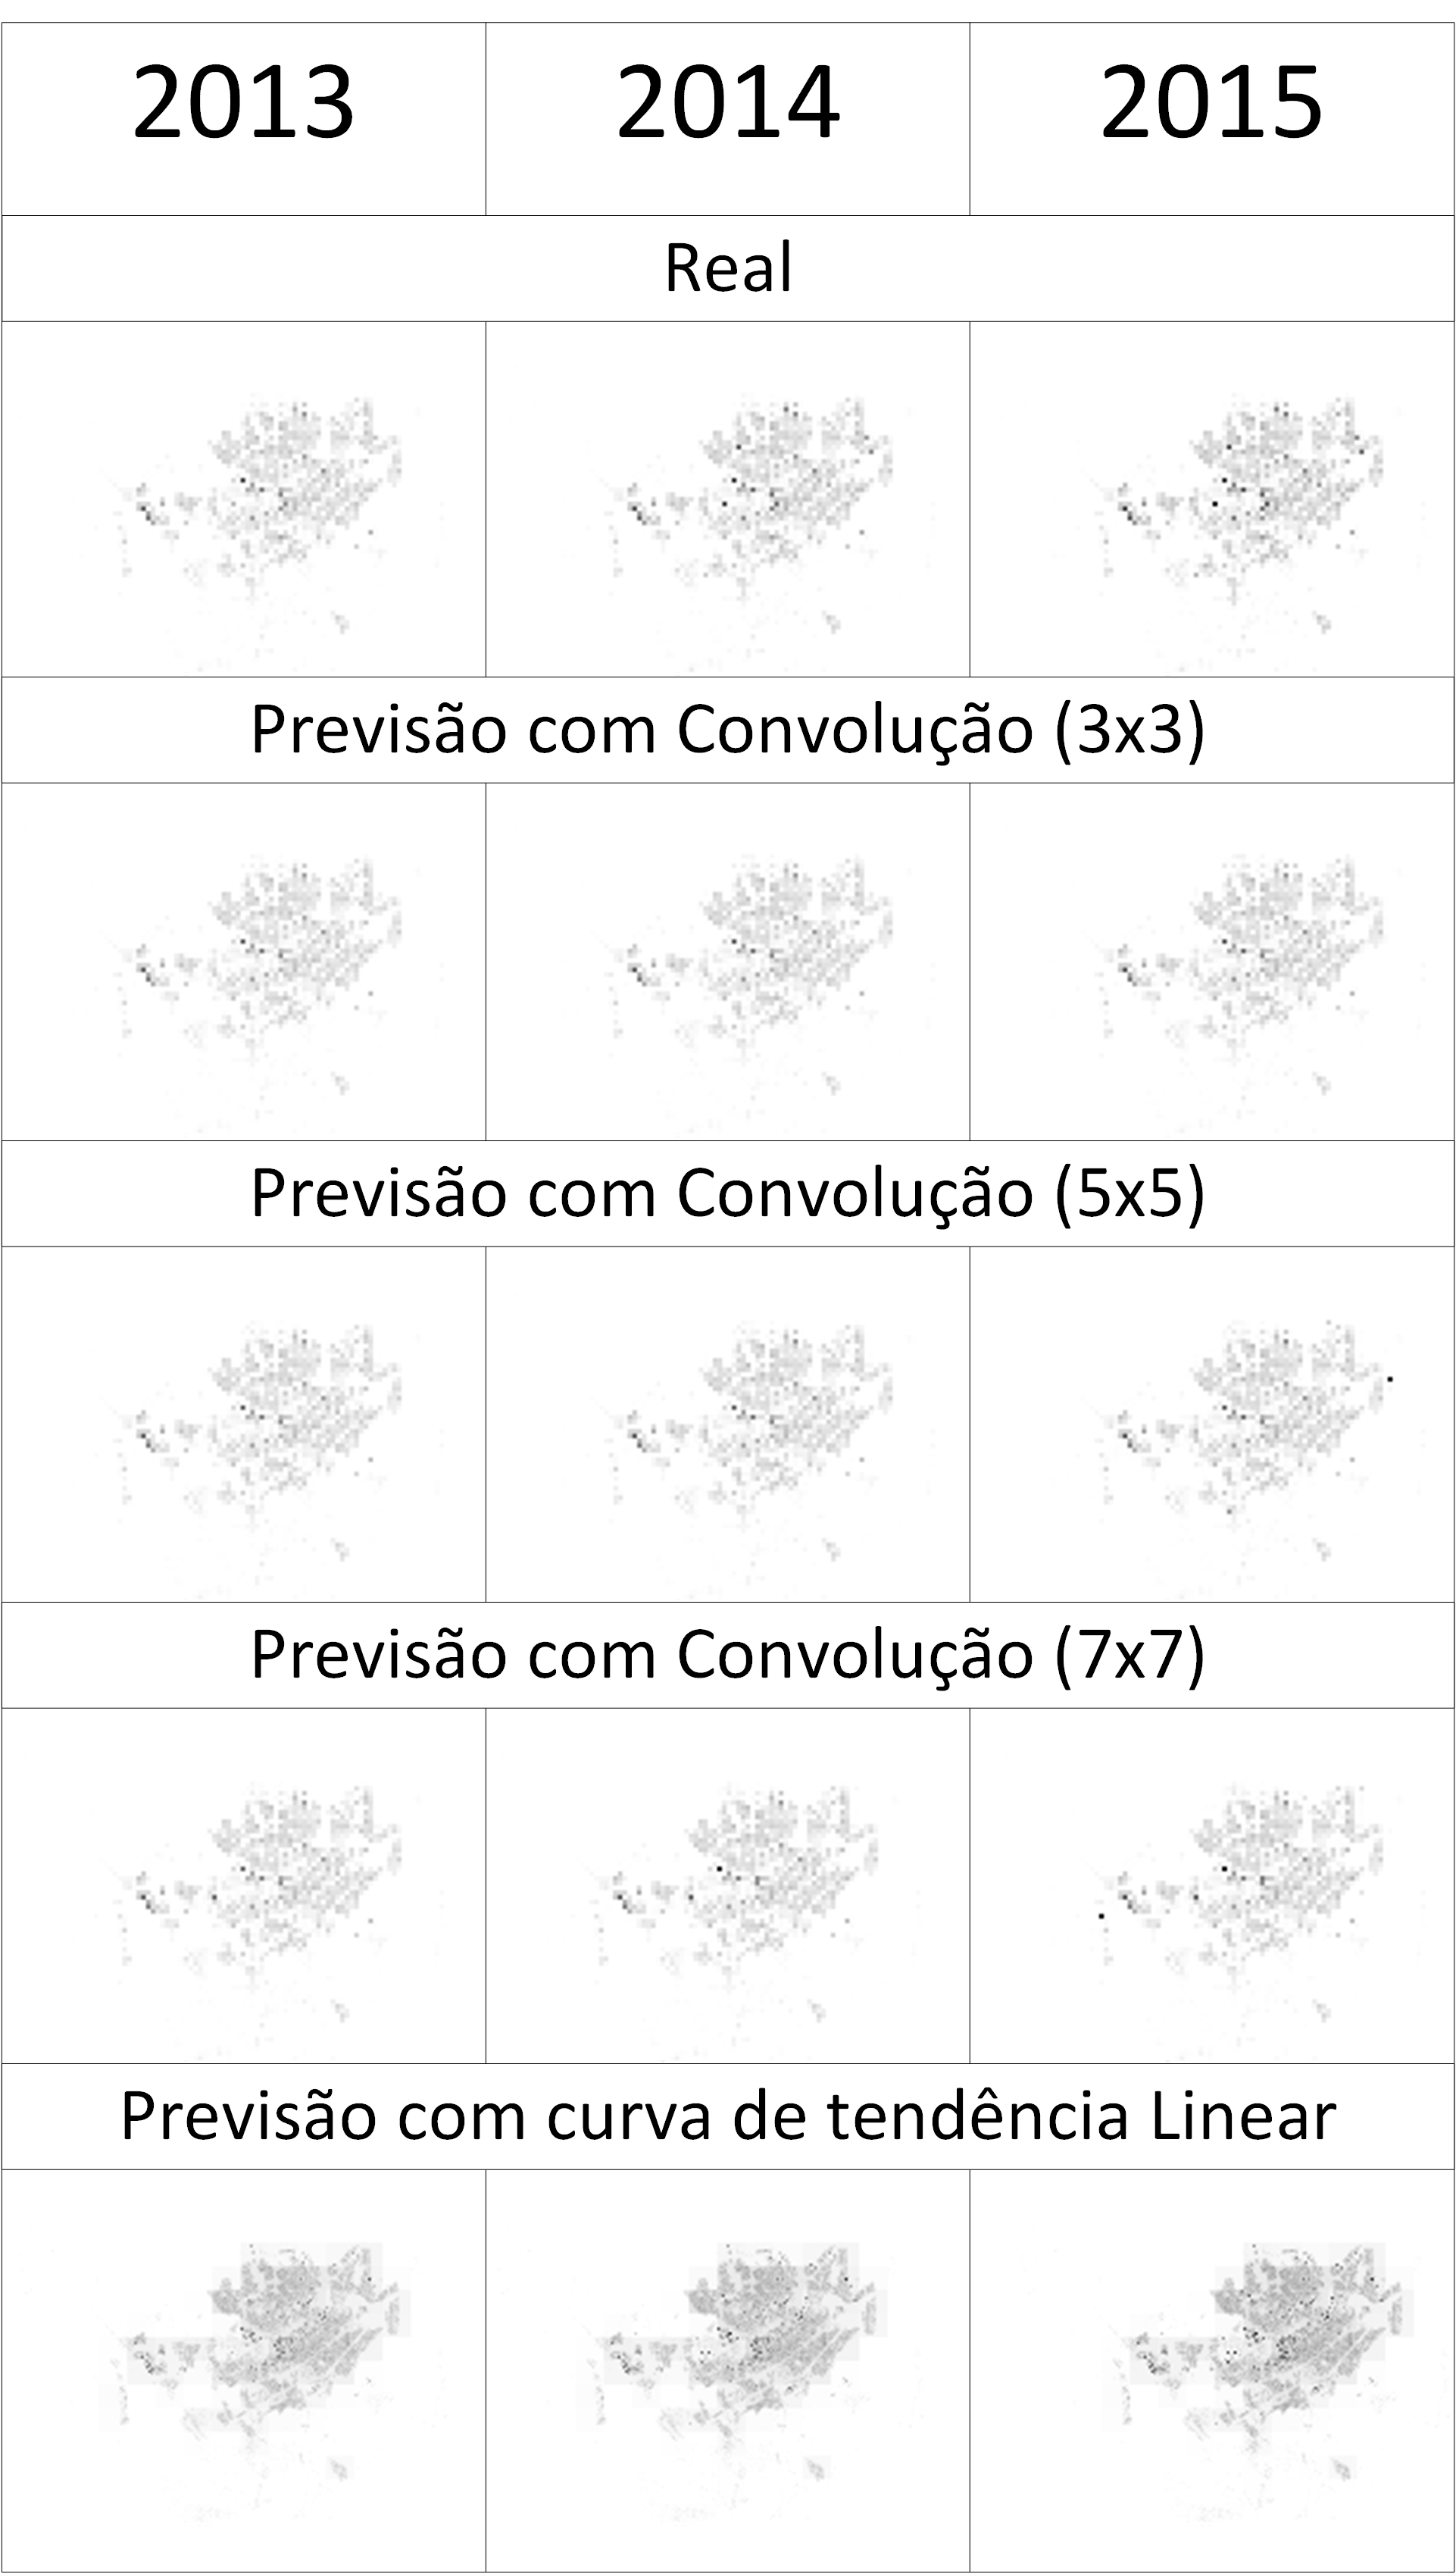
\includegraphics[scale=0.7]{Figuras/AllResults.png}
	\caption{Apresentação dos mapas reais de 2013, 2014 e 2015 comparando com a previsão por linha de tendência e com o método proposto para matrizes de convolução de ordem 3, 5 e 7}
	\label{fig:allResults}
\end{figure}

Dois parâmetros foram numericamente comparados: o erro sobre a taxa de crescimento da região prevista (Eg), e a precisão da previsão de cada célula da região (Epp). A tabela \ref{tbl:forecastErrors} mostra faz uma comparação entre os 4 métodos (proposto 3x3, proposto 5x5, proposto 7x7 e curva de tendência), onde é possível observar que o método proposto apresenta uma precisão muito semelhante em relação à linha de tendência quando compara-se o crescimento geral da região, e apresenta ainda, na previsão ponto a ponto (sobre cada célula ou \emph{pixel}) valores notavelmente melhores. Na comparação deste segundo parâmetro é possível observar ainda que ao aumentar-se a ordem da matriz de convolução não necessariamente piora-se a previsão, porém é importante notar que este aumento pode vir a extrapolar a previsão e fazer com que a precisão seja invalidada, apresentando uma previsão "estourada" como fora visto na Figura \ref{fig:ForecastingSpike}. Os valores da matriz 5x5 apresentam-se um pouco piores, devido exatamente à extrapolação na previsão do período de 2015, sendo que na Figura \ref{fig:allResults} é possível observar alguns pontos de crescimento nunca vieram a ocorrer em determinadas regiões no mapa real ou nos mapas previstos usando as matrizes de convolução de ordem 3 e 7. 

\begin{table}[h]
	\centering
	\caption{Erros de previsão}
	\label{tbl:forecastErrors}
	\begin{tabular}{l|l|l|l|l|l|}
		\cline{2-6}
		& Ano  & Eg & Eg\% & Epp & Epp\% \\ \hline
		\multicolumn{1}{|c|}{\multirow{3}{*}{Matriz 3x3}}         & 2013 & 3407,36  & 8,38\%  & 7044,81  & 2,46\%  \\ \cline{2-6} 
		\multicolumn{1}{|c|}{}                                    & 2014 & 9240,26  & 18,52\% & 14717,04 & 5,14\%  \\ \cline{2-6} 
		\multicolumn{1}{|c|}{}                                    & 2015 & 15614,48 & 26,13\% & 23649,79 & 8,27\%  \\ \hline
		\multicolumn{1}{|c|}{\multirow{3}{*}{Matriz 5x5}}         & 2013 & 3640,63  & 8,84\%  & 7359,92  & 2,57\%  \\ \cline{2-6} 
		\multicolumn{1}{|c|}{}                                    & 2014 & 9574,66  & 19,25\% & 15303,43 & 5,35\%  \\ \cline{2-6} 
		\multicolumn{1}{|c|}{}                                    & 2015 & 21038,39 & 28,86\% & 29585,02 & 10,34\% \\ \hline
		\multicolumn{1}{|c|}{\multirow{3}{*}{Matriz 7x7}}         & 2013 & 3326,51  & 8,80\%  & 7306,07  & 2,55\%  \\ \cline{2-6} 
		\multicolumn{1}{|c|}{}                                    & 2014 & 9355,60  & 18,52\% & 15325,48 & 5,36\%  \\ \cline{2-6} 
		\multicolumn{1}{|c|}{}                                    & 2015 & 16181,37 & 26,27\% & 24992,63 & 8,73\%  \\ \hline
		\multicolumn{1}{|c|}{\multirow{3}{*}{Linha de Tendência}} & 2013 & 3699,5   & 8,93\%  & 89488,3  & 31,28\% \\ \cline{2-6} 
		\multicolumn{1}{|c|}{}                                    & 2014 & 9300,8   & 18,52\% & 95026,6  & 33,21\% \\ \cline{2-6} 
		\multicolumn{1}{|c|}{}                                    & 2015 & 15757,1  & 23,15\% & 100564,9 & 35,15\% \\ \hline
	\end{tabular}
	\\[10pt]
	Nota: Validação dos resultados apresentando os erros de crescimento (Eg e Eg\%) e por pixel (Epp e Epp\%) entre o método proposto com as matrizes de convolução de ordem 3, 5 e 7 e Linha de Tendência para as previsões de 2013, 2014 e 2015
\end{table}


